\subsubsection{Assembly Line Balancing Problem}\label{subsubsec:assembly-line-balancing-problem}

Eine interessante Erweiterung des Bin Packing Problems ergibt sich durch die Einführung
von Reihenfolgebeziehungen zwischen den Objekten.

In der Literatur ist das Problem auch als Simple Assembly Line Balancing Problem (SALBP) bekannt.
Bei diesem geht es darum, eine Reihe von Aufgaben mit Vorrangbedingungen auf mehrere hintereinanderliegende
Stationen zu verteilen~\cite{alb_paper_50}.
Bei der im Folgenden betrachteten Problemvariante SALBP-1 ist die maximale Zeit für die Ausführung aller Aufgaben,
die einer Station zugeteilt werden, vorgegeben, während die Anzahl der Stationen minimiert werden soll.

Die Objekte des Bin Packing Problems sind somit nun die Aufgaben und die Behälter die Stationen des Problems.
\begin{figure}[h]
    \centering
    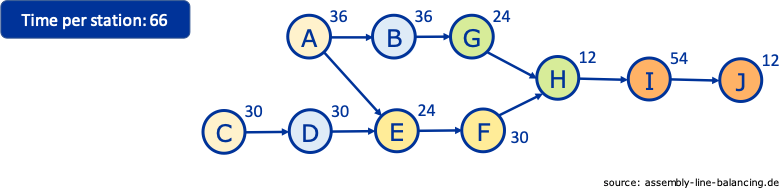
\includegraphics[width=0.8\textwidth]{images/math_problems/alb_example}
    \caption{Beispiel Assembly Line Balancing Problem und Lösung}
    \label{fig:alb_example}
\end{figure}

Als ganzzahliges Optimierungsproblem lässt sich SALBP-1 wie folgt darstellen:
Jede Aufgabe muss genau einer Station zugeteilt werden \eqref{eq:one_station_per_task}.
Pro Station muss die maximale Bearbeitungszeit eingehalten werden \eqref{eq:cycle_time_per_station}.
Die Reihenfolgebedingungen müssen eingehalten werden.
Das heißt, wenn zwischen zwei Aufgaben eine vorgegebene Reihenfolge gilt,
dann darf die zweite Aufgabe nicht auf einer Station durchgeführt werden,
die vor der der ersten Aufgabe liegt \eqref{eq:preceding_tasks}.
Das Ziel ist, die Anzahl der benötigten Stationen zu minimieren,
was mithilfe der Zielfunktion \eqref{eq:minimize_stations} erreicht wird.

\begin{table}[H]
    \begin{tabularx}{\textwidth}{  l | X | l }
    Symbol & Bedeutung & Definitionsbereich \\\hline\hline
    Mengen & & \\\hline\hline
    $T$ & Menge der Aufgaben & $\N$\\\hline
    $S$ & Menge der Stationen & $\N$\\\hline
    $R$ & Menge an Vorrangbedingungen zwischen zwei Aufgaben & $\N\times\N$\\\hline\hline
    Konstanten &  &  \\\hline\hline
    $c$ & Taktzeit & $\N$\\\hline
    $v_t$ & Benötigte Zeit für Aufgabe $t\in T$ & $\N$\\\hline\hline
    Variablen &  &  \\\hline\hline
    $x_{ts}$ & $x_{ts}=1$ gdw.\ Aufgabe $t\in T$ Station $s\in S$ zugeteilt wird & $\B$\\\hline
    $y_s$ & $y_s=1$ gdw.\ Station $s\in S$ verwendet wird & $\B$\\\hline
    \end{tabularx}
    \caption{Notation SALBP-1}\label{tab:notification}
\end{table}

\begin{align}
    \min \qquad& \sum_{s\in S} y_{s} \label{eq:minimize_stations}\\
    \textit{s.t.} \qquad
    & \sum_{s\in S} x_{ts} = 1~, \qquad &&\forall t\in T \label{eq:one_station_per_task} \\
    & \sum_{t\in T} v_{t} \cdot x_{ts} \leq c \cdot y_s~, \qquad &&\forall s\in S \label{eq:cycle_time_per_station}\\
    & \sum_{s\in S} s \cdot x_{ts} \leq \sum_{s\in S} s \cdot x_{t's}~, \qquad &&\forall (t,t')\in R \label{eq:preceding_tasks}\\
    & x_{ts}, y_s \in \B~, \qquad &&\forall t\in T, s\in S
\end{align}

\paragraph{Alternative Zielfunktionen.}
Neben den alternativen Zielfunktionen, die bereits in \cref{subsec:bin-packing} besprochen wurden,
gibt es für SALBP-1 eine weitere Möglichkeit (cf.\cite{patterson1975assembly}):
Falls es in dem durch $R$ induzierten Reihenfolgegraphen mehrere Senken gibt,
wird eine fiktive Aufgabe $t_s$ eingeführt, die nach allen anderen Aufgaben ausgeführt werden muss
($R$ muss also für alle ursprünglichen Senken $t$ um $(t,t_s)$ erweitert werden).
Da $t_s$ offensichtlich auf der letzten Station ausgeführt werden muss,
kann in der Zielfunktion die Stationsnummer dieser Aufgabe minimiert werden, um die Gesamtzahl an
Stationen zu minimieren:
\[
    \min \sum_{s\in S} s \cdot x_{st_s}
\]
Im Hinblick auf die Minimierung der benötigten Variablen und Constraints könnte diese Formulierung dann hilfreich sein,
wenn es in einer konkreten SALBP-1 Instanz bereits wenig Senken im Reihenfolgegraphen gibt
und potentiell viele Stationen benötigt werden (wodurch die ursprüngliche Formulierung viele $y$ Variablen erfordern würde).